\chapter{Softwarekonzept} \label{chap:Konzept}

Dieser Studienarbeit liegt der, in der letzten Studienarbeit beschriebene Code, zugrunde. Dieser wurde im Rahmen einer Machbarkeitsstudie entwickelt und untersucht.
Zentraler Fokus des Softwarekonzepts liegt auf der Präsentierparkeit und Wiederverwenbarkeit dieser Machbarkeitsstudie als Anwendung für die FESTO \ac{cp-lab}.

Um eine größere Auswahl an Möglichkeiten, sowie eine bessere Kontrolle über die Software zu erhalten, wird die Software in eine lokale Umgebung verschoben. Zusätzlich sollen alle einstellbaren Parameter zentral aufgeführt werden. Dies ermöglicht eine einfache Konfiguration der Software und entspricht dem Stand der Technik\cite{gur_diskussion_2024} \cite{oliveira_how_2023}. 

\section{Programmstruktur} \label{sec:architektur}

Erster Teil der Softwarekonzeption ist der Entwurf der Struktur. Die Struktur einer Software ist entscheidend für die Wartbarkeit und Erweiterbarkeit. Zwei zentrale Kriterien, deren Erhaltung im gesamten Entwurfsprozess berücksichtigt werden muss.

\begin{figure}[H]
    \centering
    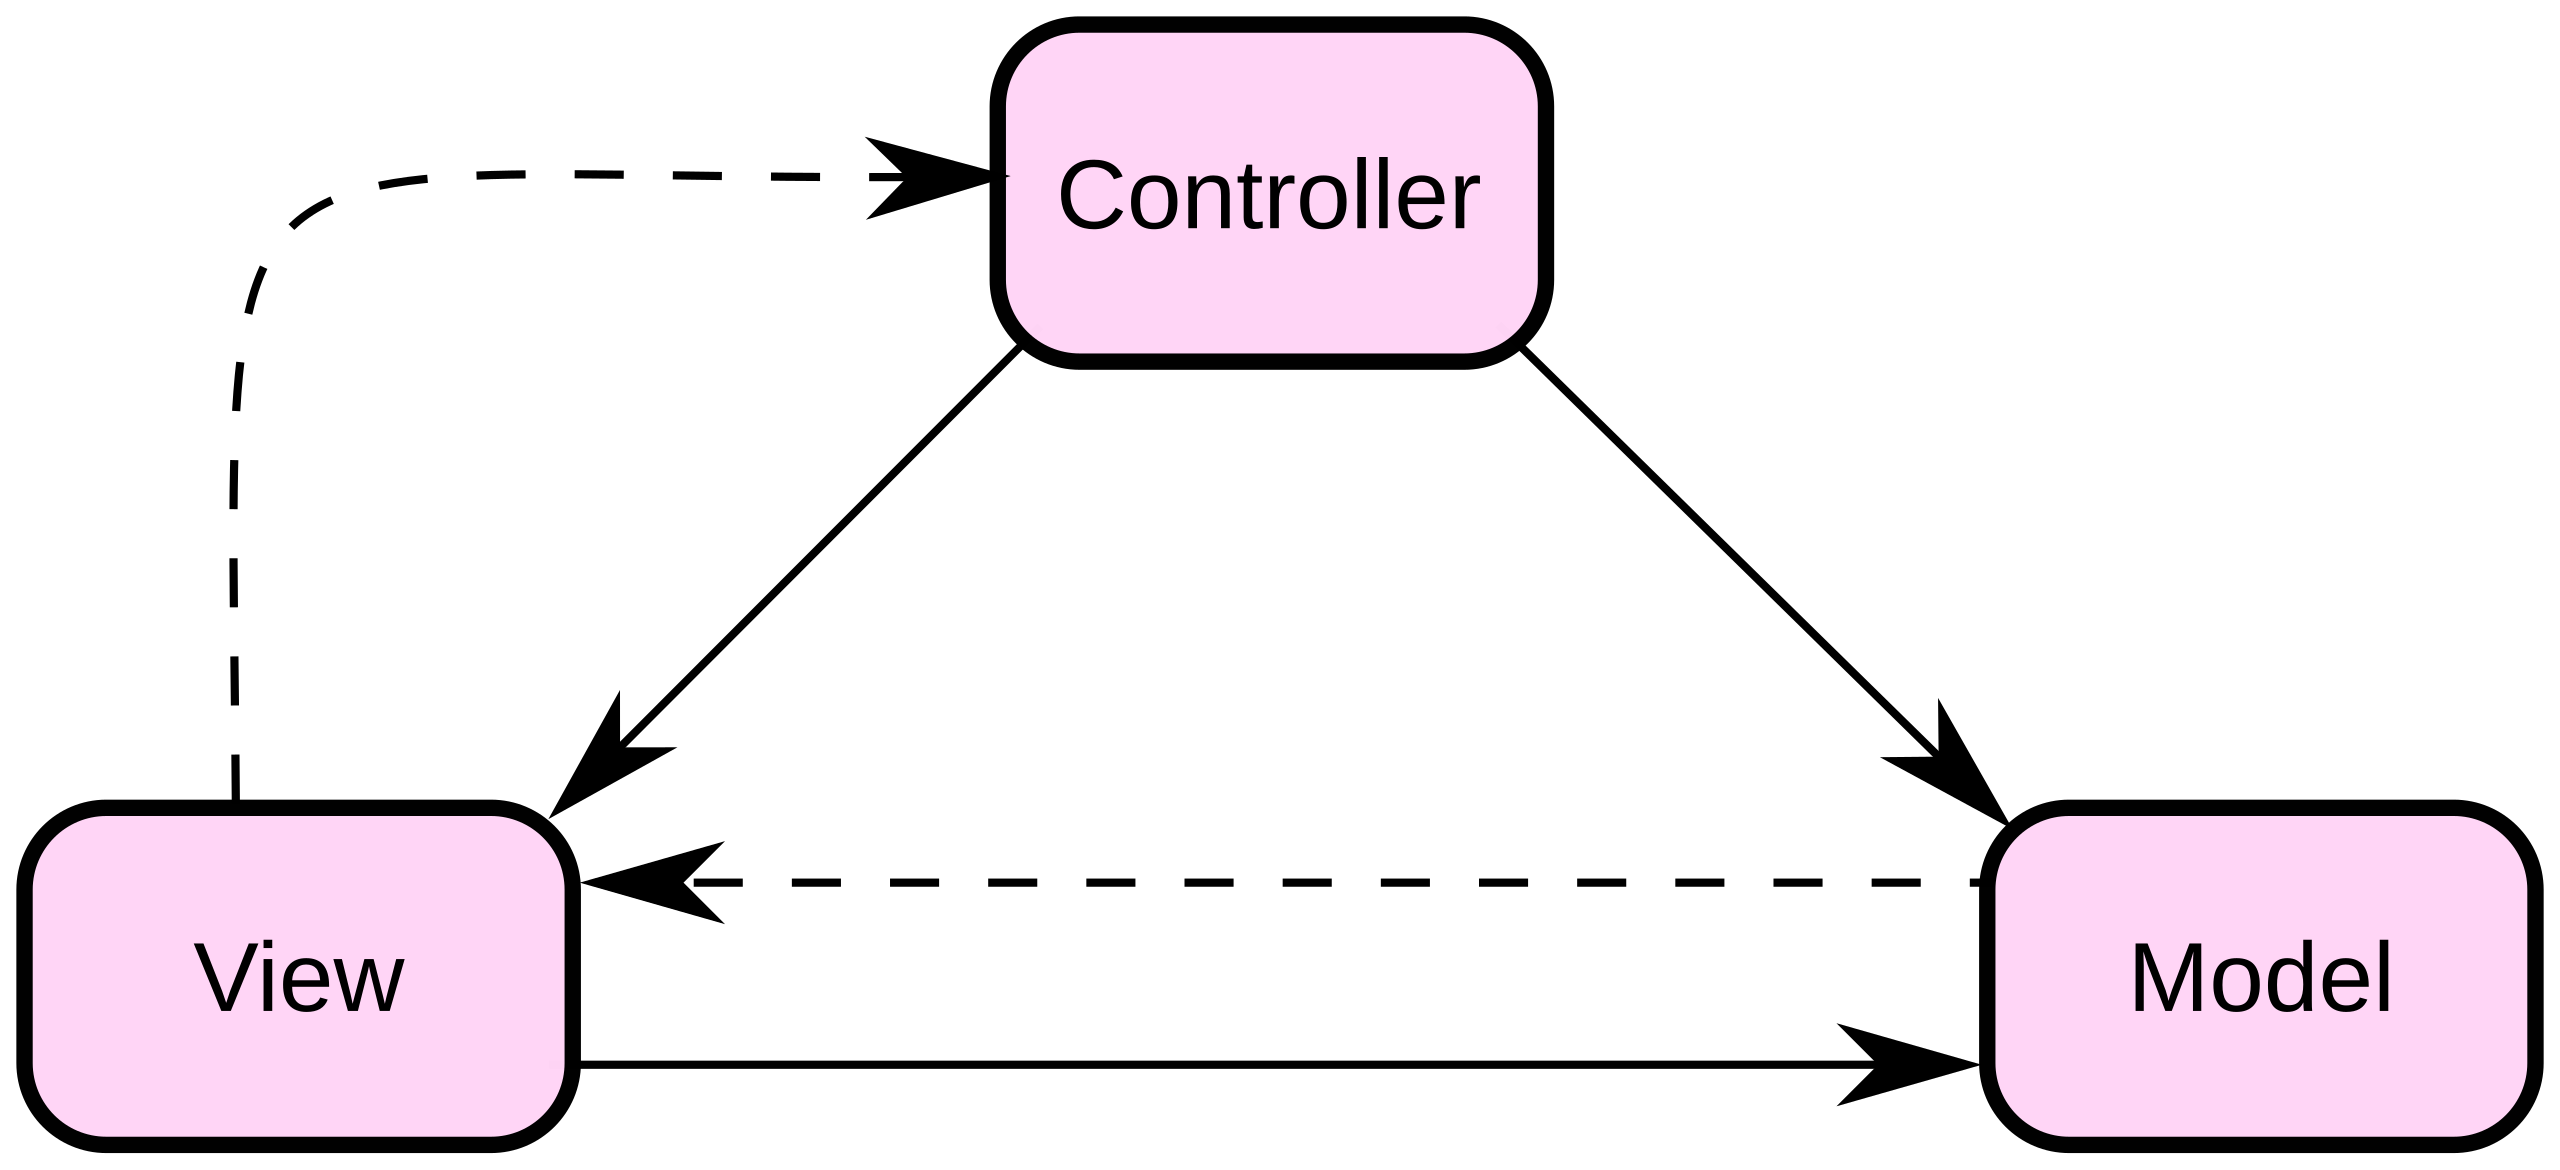
\includegraphics[width=0.8\textwidth]{MVC_struktur.png}
    \caption{Schematische Darstellung der MVC Struktur \cite{noauthor_model_2024}} 
    \label{fig:MVC_struktur}
\end{figure}

Im Rahmen dieser Studienarbeit gibt es keine externen Anforderungen an die Struktur. Daher wurde sich für eine vereinfachte \ac{MVC} Struktur entschieden (\autoref{fig:MVC_struktur}). Ziel dieser Struktur ist es die Software in drei Teile zu unterteilen.
Diese drei Teile sollen eigenständige Aufgaben übernehmen und so verhindern, dass das Programm zu einem monolithischen Codeblock wird.

Der Model-Teil ist für die (Bild-) Datenverarbeitung zuständig und enthält die Datenstrukturen sowie die Logik, die die Daten verarbeitet. Der View-Teil ist für die Darstellung der Daten verantwortlich und umfasst die Benutzeroberfläche sowie die Logik, die die Daten darstellt. Der Controller-Teil steuert die Daten und koordiniert die Kommunikation zwischen Model und View, indem er die entsprechende Logik enthält.

Die vereinfachte Version der \ac{MVC} Struktur kombiniert die Funktionalitäten von View und Controller in der \ac{API} (Siehe \autoref{fig:MVC_struktur}) und trennt die Datenverarbeitung in einem eigenes Modul ab. Dieses eigene Modul wird im Programmcode \texttt{Pycore} genannt und enthält die Funktionen, welche die Daten für das Neuronale Netzwerk aufbereiten und zur Verfügung stellen.

\section{Konfiguration der Programmparameter} \label{sec:konfiguration}

Aus der Aufgabenstellung (siehe \autoref{sec:problemstellung_und_ziel_dieser_arbeit}) lässt sich ein weiterer Teil des Softwarekonzepts, die Einstellbarkeit, ableiten.
Durch die Einstellbarkeit soll gewährleistet sein, dass die Software flexibel an die Anforderungen des Benutzers angepasst werden kann, ohne dass der Benutzer ein tiefes Verständnis der Software haben muss.

\begin{figure}[H]
    \centering
    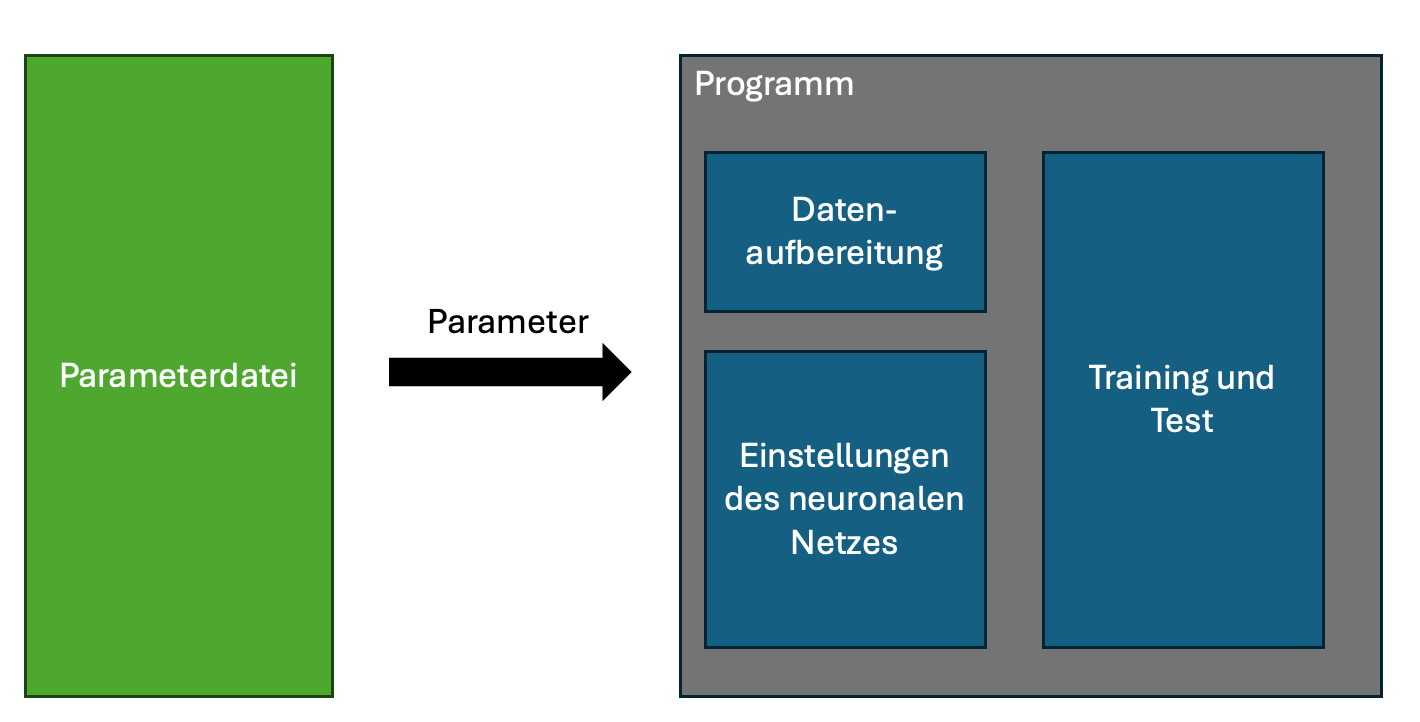
\includegraphics[width=0.8\textwidth]{Parameterverteilung.png}
    \caption{Konzept der Parametergruppierung- und Verteilung auf das Programm} 
    \label{fig:json_example}
\end{figure}

Ziel ist es das der Benutzer eine einzige Datei öffnet und dort alle Einstellungen vornehmen kann. 
Diese Datei soll im \ac{JSON}-Format vorliegen, da es ein weit verbreitetes Format ist und von vielen Programmiersprachen unterstützt wird \cite{gur_diskussion_2024}.


\section{Die Weboberfläche mittels Python Web API} \label{sec:weboberflaeche}

Das zentrale Element des neuen Programmentwurfs stellt die Webanwendung dar. Dieses neue Interface zwischen Benutzer und Programm ermöglicht es neue Bilder des FESTO \ac{cp-lab} darzustellen, zu klassifizieren und die Ergebnisse auf seiner Weboberfläche visualisieren.
Zusätzlich koordiniert sie die Überwachung des Ordners für neue Bilder und die Klassifizierung dieser Bilder in Defekt oder nicht Defekt.

\begin{figure}[H]
    \centering
    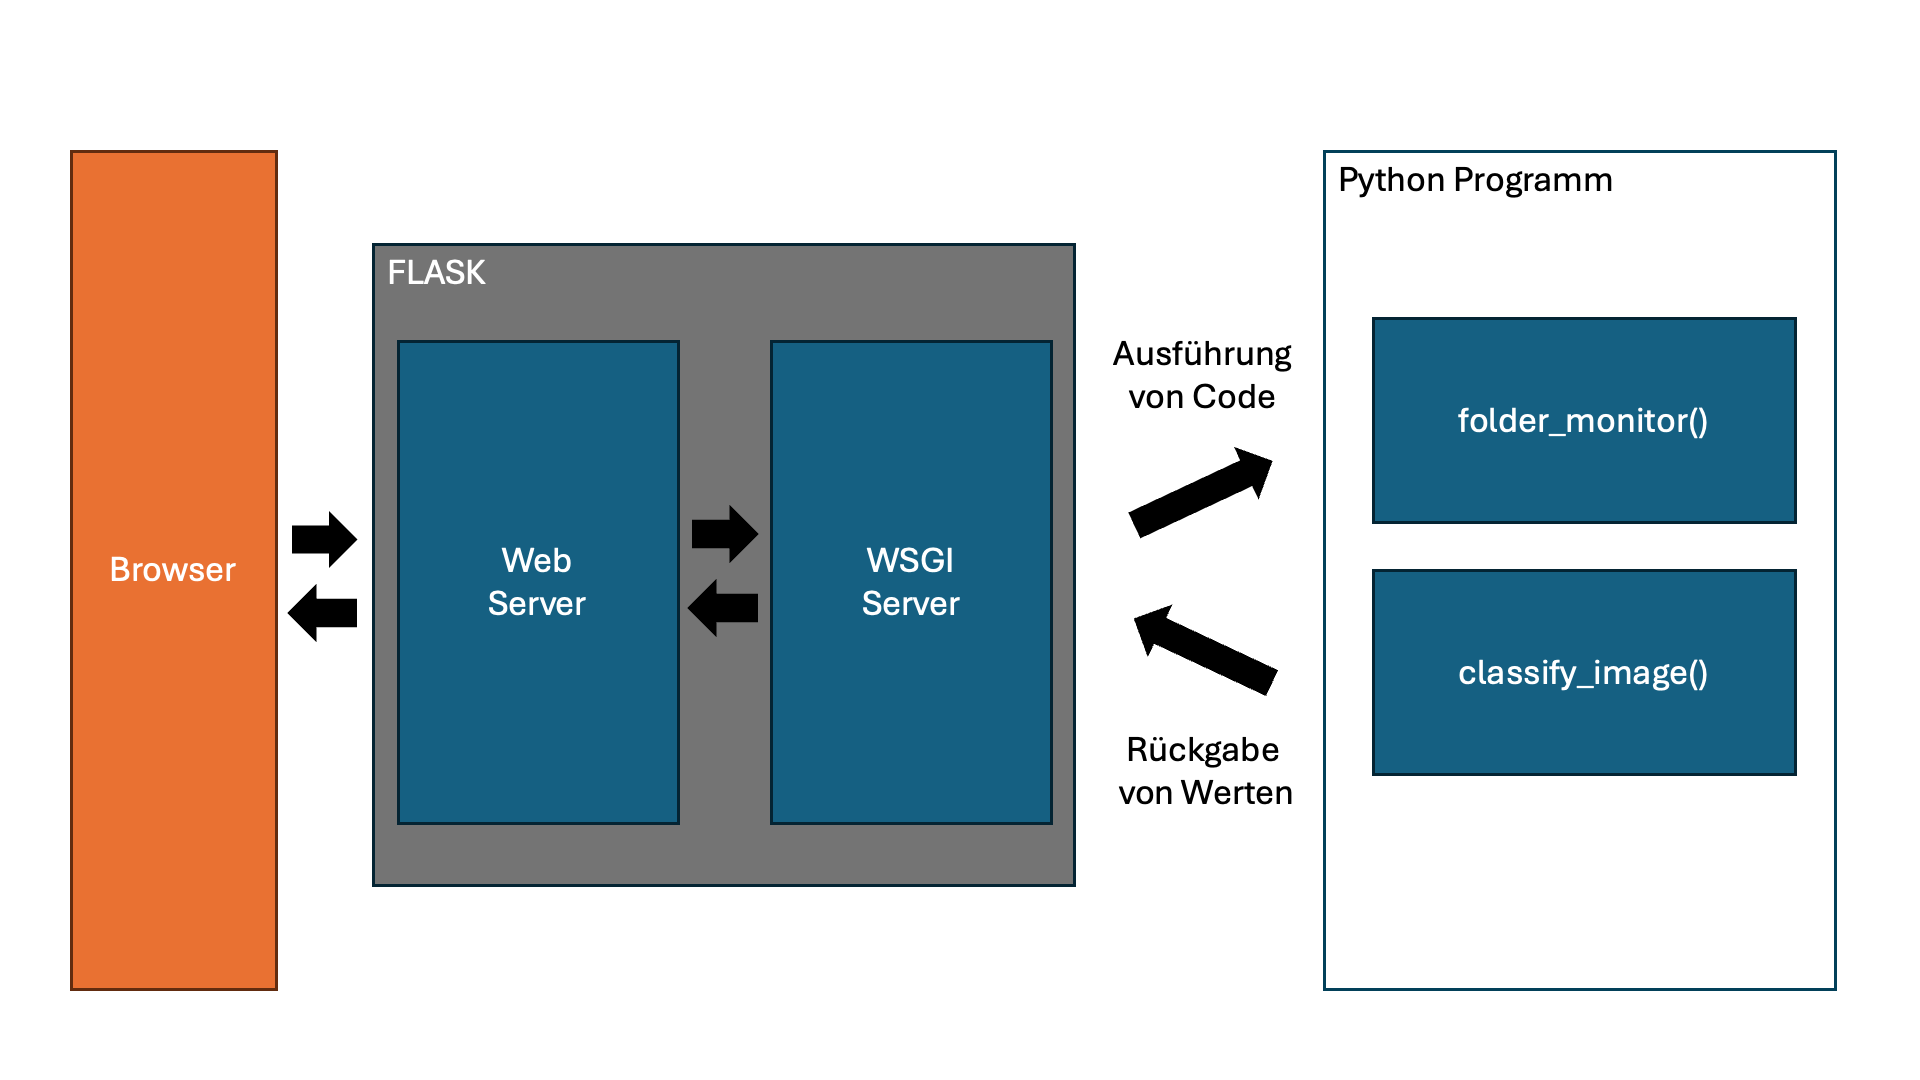
\includegraphics[width=0.8\textwidth]{API_Python_func.png}
    \caption{Aufschlüsselung der API Funktionen} 
    \label{fig:Api_funktionen}
\end{figure}

Der Aufbau des Programmteils folgt dem funktionalen Prinzip einer \ac{API}, welche in \autoref{sec:api} beschrieben ist. Die \autoref{fig:Api_funktionen} erweitert die \autoref{fig:flask} um die beiden Haputfunktionen, welche die API innerhalb des Python Programmes ausführt. Der Benutzer wird in der Lage sein das aktuelle Werkstück im Browser zu sehen, ohne sich mit dem Programmcode auseinandersetzen zu müssen. Hierfür sollen parallel mehrere Prozesse gestartet werden, welche die API, überwachung des Ordners und klassifizierung des aktuellen Bildes übernehmen.